\providecommand\IfDocumentMetadataT[1]{}
\providecommand\IfDocumentMetadataTF[2]{#2}
\documentclass[a4paper,fleqn]{cas-dc}

\usepackage{amsmath}
\usepackage{booktabs}
\usepackage{array}
\usepackage{tikz}
\usepackage[numbers]{natbib}
\usetikzlibrary{arrows.meta,positioning,calc}
\emergencystretch=2em
\ExplSyntaxOn
\RenewDocumentCommand \printorcid {} {}
\ExplSyntaxOff

\begin{document}
\let\WriteBookmarks\relax
\def\floatpagepagefraction{1}
\def\textpagefraction{.001}

\shorttitle{Constraint-Graph Policy Optimizer}
\shortauthors{Anonymous}

\title[mode=title]{Constraint-Graph Policy Optimizer for Constrained Multi-UAV Multi-Objective Path Planning}

\author[1]{Anonymous Author}
\affiliation[1]{organization={Anonymous for review},
                city={Review copy},
                country={Submission manuscript}}

\begin{abstract}
Multi-UAV path planning is a constrained multi-objective optimization problem in which path quality, terrain clearance, kinematic feasibility, and inter-UAV separation must be considered together. Recent UAV planning and benchmarking studies emphasize realistic environment classes, fixed protocols, named baselines, statistical analysis, and reproducibility artifacts. However, many evolutionary UAV planners still treat constraint ranking, parent selection, and fleet-aware variation as weakly connected rules, making it difficult to inspect how observed violations influence search behavior. This paper presents the Constraint-Graph Policy Optimizer (CGPO), a lean graph-guided evolutionary optimizer for constrained multi-UAV path planning. CGPO builds a dynamic constraint-interaction graph over candidate fleet paths and uses the resulting tension signals in three coupled mechanisms: constraint-interaction graph construction (CIG), Pareto pressure-field selection (PPF), and orchestrated fleet variation (OVO). The active repository implementation contains no explicit repair stack, no graph-guided feasibility projection module, no constructive route-prior baseline, and no matched CGPO hybrid algorithms; all candidate improvement is performed through population-based evolutionary selection and variation with domain-bound clipping. A reduced matched evaluation on city, mountain, and suburban fleet-three cases uses population 40, 500 generations, five independent runs, matched safety constraints, hypervolume, IGD+, feasibility, mission diagnostics, and runtime. In this reduced protocol, CGPO is feasible in all 15 matched runs, achieves the best scenario-level HV rank, and outperforms NSGA-II, MOEA/D, and NMOPSO on matched run-level HV comparisons under Holm-corrected Wilcoxon tests. Focused inspection and ablation runs further verify fleet-size behavior and traceable CIG, PPF, and OVO switches. The contribution is a reproducible evolutionary graph-based optimizer and a journal-style reduced evaluation package for testing whether graph-derived constraint pressure improves constrained multi-UAV search.
\end{abstract}

\begin{keywords}
multi-UAV path planning \sep multi-objective optimization \sep constrained evolutionary optimization \sep constraint handling \sep benchmark protocol \sep hypervolume \sep feasibility diagnostics
\end{keywords}

\maketitle

\section{Introduction}
\label{sec:introduction}

Unmanned aerial vehicles (UAVs) are increasingly used in tasks such as inspection, delivery, mapping, surveillance, and reconnaissance. In these settings, path planning is not only a shortest-path problem. A usable route must balance travel efficiency with terrain clearance, altitude restrictions, smoothness, energy-related cost, and safety margins \cite{jiang2024ec_uav_survey,besada2013uav_comparison,darlan2025benchmark}. The difficulty increases further when several UAVs fly in a shared environment, because each path can create pairwise separation constraints and timing-dependent conflicts for the rest of the fleet \cite{zhang2024twofold_uav,meng2025emmop}.

Multi-objective formulations are a natural fit for this setting because improving one criterion can degrade another. A path that shortens distance may pass closer to terrain or other UAVs. A path that increases clearance may require sharper turns or more energy. Prior UAV path-planning studies and benchmark papers therefore evaluate algorithms using multiple objectives and safety diagnostics rather than a single scalar route cost \cite{peng2022decomp_uav,darlan2025benchmark,meng2025emmop,zhou2024tskac,duong2025nmopso_uav}.

Despite this progress, constrained multi-UAV planning still has a control problem inside the optimizer. Evolutionary and swarm planners often combine archives, constraint ranking, crossover, and mutation through separate rules. This can produce useful results, but it weakens the connection between the constraints observed during search and the operators used to modify candidate paths. In particular, a selection mechanism may suppress infeasible candidates without distinguishing harmful violations from useful near-boundary candidates, and a variation operator may alter one UAV path without considering its fleet-level coupling.

This paper addresses that gap with CGPO, a Constraint-Graph Policy Optimizer for constrained multi-UAV multi-objective path planning. CGPO uses one dynamic constraint-interaction graph to summarize terrain, altitude, turn-angle, pairwise-separation, and path-smoothing tension. The graph then drives parent-selection pressure and coordinated offspring generation. The current method is intentionally kept as a lean evolutionary algorithm: it does not use explicit repair, graph-guided feasibility projection, constructive A$^\star$ route priors, or matched hybrid baselines. The intent is to make constraint pressure visible both to the optimizer and to the result analysis rather than to hide feasibility behind a post-processing step.

The key contributions are summarized as follows:
\begin{enumerate}
\item A constraint-interaction graph representation for fleet candidate paths that exposes terrain, altitude, turn-angle, pairwise-separation, and path-smoothing tension as recorded graph summaries.
\item A lean graph-guided evolutionary optimizer that couples constraint-interaction graph construction, Pareto pressure-field selection, and orchestrated fleet variation in one population-based search loop.
\item A reproducible SWEC-style evaluation protocol for constrained multi-UAV path planning, with fixed terrain cases, fleet sizes, budgets, baselines, safety diagnostics, hypervolume, IGD+, runtime, statistical analysis, and ablation variants.
\item A completed reduced matched comparison showing CGPO feasibility and HV advantages against NSGA-II, MOEA/D, and NMOPSO under the 40-population, 500-generation, five-run protocol, plus focused fleet-size and ablation inspections.
\end{enumerate}

The remainder of the paper is organized as follows. Section \ref{sec:related-work} reviews related work on UAV path planning, benchmark design, constrained evolutionary optimization, and structure-aware search. Section \ref{sec:problem} formulates the benchmark problem. Section \ref{sec:method} describes CGPO. Section \ref{sec:experimental-protocol} gives the experimental protocol. Sections \ref{sec:results} and \ref{sec:ablation} report the reduced matched comparison, focused validation evidence, ablation results, and trace analysis. Sections \ref{sec:reproducibility} and \ref{sec:limitations} describe reproducibility and limitations. Section \ref{sec:conclusion} concludes.

\section{Related work}
\label{sec:related-work}

\subsection{Multi-objective UAV path planning}

UAV path planning has been studied with graph search, sampling methods, potential fields, swarm intelligence, and evolutionary computation \cite{jiang2024ec_uav_survey}. For complex environments, multi-objective approaches are useful because decision makers often need a set of trade-off paths rather than one weighted-sum solution. Early comparative work emphasized the need for problem-specific quality indicators and statistical characterization when comparing multi-objective UAV planners \cite{besada2013uav_comparison}. More recent benchmark work frames UAV path planning around conflicting safety, efficiency, and regulatory constraints and introduces standardized urban, suburban, and mountainous scenarios \cite{darlan2025benchmark}.

Recent multi-UAV work strengthens the same direction. Two-fold constraint handling has been studied for multiple-UAV path planning \cite{zhang2024twofold_uav}; knowledge-assisted coevolution has been used for bi-objective multi-UAV planning \cite{zhou2024tskac}; and evolutionary multitasking has been used for multiobjective multi-UAV path planning with adaptive operator selection and knowledge fusion \cite{meng2025emmop}. These works motivate the present paper's fleet setting: single-UAV path quality is insufficient when inter-UAV constraints become part of the mission.

\subsection{Benchmarking and reproducible comparison}

Benchmark papers in this area emphasize shared environments, fixed protocols, and clear baseline roles. Darlan et al. \cite{darlan2025benchmark} explicitly argue that inconsistent scenarios and inaccessible code make algorithm comparison difficult. This repository follows that benchmark direction by using named protocol files, benchmark manifests, per-run artifacts, metrics summaries, and a separation between benchmark-safe algorithms and experimental research methods.

For CGPO, this matters because the algorithm is experimental. The manuscript therefore separates the method proposal from the comparative claim. The method can be described from code, but performance claims require the locked protocol outputs. The main, ablation, and single-UAV reference protocols are named YAML configs under \texttt{configs/}.

\subsection{Constrained evolutionary optimization}

Constrained multi-objective optimization requires algorithms to handle objective trade-offs and constraint satisfaction simultaneously. Constraint-handling surveys and recent constrained MOEA work show that feasibility ranking, archives, auxiliary tasks, push-pull strategies, two-archive designs, and multitasking can all influence search behavior \cite{mezura2011constraint_survey,ming2024emt_cmop,yu2024constraint_emt}. The CGPO design is closest to constraint-handling methods that treat infeasible and boundary candidates as informative rather than simply invalid.

The difference is representational. CGPO does not only compute a scalar constraint violation. It builds a constraint-interaction graph over route waypoints and uses the graph's tension field to guide selection pressure and variation. This lets the method record internal signals such as mean tension, pairwise edge count, smoothing edge count, conflict-cluster count, pressure entropy, perturbation scale, and coordinated clusters.

\subsection{Baseline algorithm families}

The paper uses an online/offline baseline scope. Here, online means that the method is part of the active comparison narrative or benchmark protocol; it does not mean real-time online replanning. Offline methods are retained as background, historical artifacts, or deferred comparators and are not used for headline numerical claims.

Table \ref{tab:baseline-online-scope} lists the online algorithm set. NSGA-II is included as a canonical elitist multi-objective evolutionary algorithm \cite{deb2002nsga2}. MOEA/D is used as a decomposition-style convergence baseline. NMOPSO represents the UAV path-planning PSO family, consistent with recent UAV PSO formulations \cite{duong2025nmopso_uav}. MOEA-2DE and EMMOP represent UAV-specialized external reference-code methods. TSKAC-NSGA-II represents a UAV-specialized multi-UAV coevolutionary baseline related to knowledge-assisted planning \cite{zhou2024tskac}. CCEA-ADVS is kept in the MOEA-style online paper scope as a multi-UAV coevolution reference. DTAPP-IICR is kept as a separate MAPF/preflight coordination baseline because it returns a coordinated fleet plan rather than a Pareto population.

\begin{table*}[t]
\centering
\scriptsize
\caption{Online algorithm scope for the paper. Online denotes active paper scope, not dynamic real-time replanning.}
\label{tab:baseline-online-scope}
\setlength{\tabcolsep}{3pt}
\begin{tabular*}{\textwidth}{@{\extracolsep{\fill}}p{0.15\textwidth}p{0.12\textwidth}p{0.34\textwidth}p{0.27\textwidth}}
\toprule
Scope & Algorithm & Core mechanism & Paper role \\
\midrule
Generic MOEA & \texttt{NSGA-II} & Pareto sorting and crowding distance & Standard MOEA baseline \\
Generic MOEA & \texttt{MOEAD} & Weight-vector decomposition & Convergence-oriented baseline \\
UAV-specific MOEA & \texttt{NMOPSO} & Navigation-variable PSO with kinematic constraints & UAV path-planning baseline \\
UAV-specific MOEA & \texttt{MOEA-2DE} & Dimension exploration and discrepancy evolution & Single-UAV reference-code comparator \\
UAV-specific MOEA & \texttt{EMMOP} & Evolutionary multitasking and knowledge transfer & Single-UAV reference-code comparator \\
Constraint handling & \texttt{NSGA-II} with Deb rules & Feasibility-first constraint domination & Constrained-search baseline \\
Multi-UAV optimization & \texttt{CCEA-ADVS} & Co-evolutionary decomposition & Deferred fair-wiring target \\
Multi-UAV optimization & \texttt{TSKAC-NSGA-II} & Two-stage cooperative optimization & Runnable multi-UAV baseline \\
Separate MAPF & \texttt{DTAPP-IICR} & Delivery-time prioritized planning with iterative conflict resolution & Preflight coordination reference, reported separately \\
\bottomrule
\end{tabular*}
\end{table*}

All other algorithms are offline for the current manuscript scope. This includes L-SHADE-CDP, C-TAEA, GCNMOEA, MO-MFEA-II, MOEAD-AWA-ASTAR, the legacy SAC/relational-state variants, and custom MOGWO variants. They may be discussed as related work or future comparator targets, but no headline numeric comparison is reported for them in this manuscript unless the protocol is explicitly expanded.

\section{Problem formulation}
\label{sec:problem}

\subsection{Environment and candidate representation}

The benchmark represents an environment as a terrain map with horizontal bounds, altitude limits, and scenario-specific obstacle or terrain structure. The active CGPO/SWEC protocol uses the \texttt{paper\_medium} scenario set with three named cases: \texttt{c\_100}, \texttt{m\_100}, and \texttt{s\_120}. These correspond to the city, mountain, and suburban terrain families used by the repository's benchmark workflow.

A fleet candidate is a set of waypoint paths
\begin{equation}
X=\{P_1,\ldots,P_m\}, \qquad
P_u=(x_{u,i},y_{u,i},z_{u,i})_{i=1}^{n},
\end{equation}
where $m$ is the fleet size and each path has fixed start and goal endpoints. CGPO modifies internal waypoints only. This keeps the optimization focused on route shape and fleet interaction rather than changing the mission definition.

\subsection{Objectives and diagnostics}

The repository evaluator reports four objective channels through the common UAV benchmark pipeline. The manuscript intentionally does not rename these channels into unsupported physical quantities beyond the repository documentation; they are treated as path-quality, terrain/altitude, smoothness or mission-quality, and safety-related objective channels. In addition, the metrics pipeline reports feasible ratio, run success, hypervolume (HV), IGD+, runtime, minimum clearance, maximum turn angle, mission conflict rate, mission makespan, and mission energy.

HV and IGD+ measure Pareto-set quality, while the mission diagnostics prevent unsafe paths from being hidden behind aggregate objective scores. This follows the evidence style of SWEC UAV papers, where tables, convergence, path visualizations, and safety diagnostics are used together rather than relying on one metric.

\subsection{Constraints}

The registered protocol fixes the mission constraints shown in Table \ref{tab:constraints}. Feasibility is determined by the shared mission evaluator and constraint-violation machinery used by the benchmark. The main hard constraints are terrain clearance, altitude bounds, turn-angle limits, and inter-UAV separation. The same evaluator is used for CGPO and non-CGPO baselines in the benchmark workflow.

\begin{table}[t]
\centering
\small
\caption{Mission constraints fixed by the registered protocol.}
\label{tab:constraints}
\begin{tabular}{lrl}
\toprule
Parameter & Value & Evidence source \\
\midrule
\texttt{separationMin} & 10.0 & Head-to-head config \\
\texttt{maxTurnDeg} & 75.0 & Head-to-head config \\
\texttt{safeDist} & 20.0 & Head-to-head config \\
\texttt{droneSize} & 1.0 & Head-to-head config \\
\texttt{hardCollisionConstraint} & true & Head-to-head config \\
\bottomrule
\end{tabular}
\end{table}

\section{Method: Constraint-Graph Policy Optimizer}
\label{sec:method}

\subsection{Design rationale}

The central design decision in CGPO is to make constraint pressure inspectable before it is used. Terrain, altitude, turn, pairwise, and path-smoothing pressures are converted into a graph-based tension field. The optimizer then uses this field in two places: selection and variation. CGPO deliberately avoids explicit repair and graph-guided feasibility projection in the active method, so any observed improvement must come from evolutionary search pressure rather than from a separate correction layer. If a mechanism does not help, the ablation protocol should expose it.

\begin{figure*}[t]
\centering
\resizebox{\textwidth}{!}{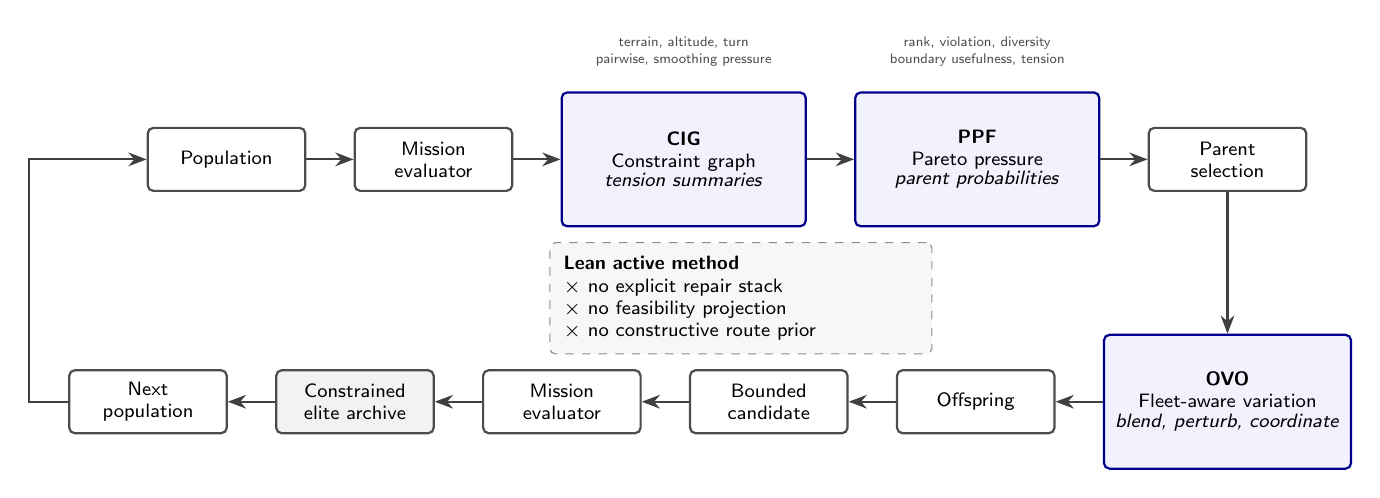
\begin{tikzpicture}[
  font=\sffamily\scriptsize,
  >=Stealth,
  stage/.style={
    rectangle,
    draw=black!70,
    thick,
    rounded corners=2pt,
    align=center,
    minimum height=8mm,
    minimum width=20mm,
    inner xsep=4pt,
    inner ysep=4pt,
    fill=white
  },
  mechanism/.style={
    stage,
    draw=blue!55!black,
    fill=blue!5,
    minimum width=31mm,
    minimum height=17mm
  },
  note/.style={
    rectangle,
    draw=black!45,
    dashed,
    rounded corners=2pt,
    align=left,
    fill=gray!6,
    inner sep=5pt,
    text width=45mm
  },
  flow/.style={->, thick, draw=black!75},
  hint/.style={font=\sffamily\tiny, text=black!70, align=center, text width=31mm}
]

\node[stage] (pop) {Population};
\node[stage, right=6mm of pop] (evalA) {Mission\\evaluator};
\node[mechanism, right=6mm of evalA] (cig) {\textbf{CIG}\\Constraint graph\\[-1pt]\textit{tension summaries}};
\node[mechanism, right=6mm of cig] (ppf) {\textbf{PPF}\\Pareto pressure\\[-1pt]\textit{parent probabilities}};
\node[stage, right=6mm of ppf] (parents) {Parent\\selection};

\node[mechanism, below=18mm of parents] (ovo) {\textbf{OVO}\\Fleet-aware variation\\[-1pt]\textit{blend, perturb, coordinate}};
\node[stage, left=6mm of ovo] (offspring) {Offspring};
\node[stage, left=6mm of offspring] (bounded) {Bounded\\candidate};
\node[stage, left=6mm of bounded] (evalB) {Mission\\evaluator};
\node[stage, fill=gray!10, left=6mm of evalB] (archive) {Constrained\\elite archive};
\node[stage, left=6mm of archive] (next) {Next\\population};

\draw[flow] (pop) -- (evalA);
\draw[flow] (evalA) -- (cig);
\draw[flow] (cig) -- (ppf);
\draw[flow] (ppf) -- (parents);
\draw[flow] (parents) -- (ovo);
\draw[flow] (ovo) -- (offspring);
\draw[flow] (offspring) -- (bounded);
\draw[flow] (bounded) -- (evalB);
\draw[flow] (evalB) -- (archive);
\draw[flow] (archive) -- (next);
\draw[flow] (next.west) -- ++(-5mm,0) |- (pop.west);

\node[hint, above=2mm of cig] {terrain, altitude, turn\\pairwise, smoothing pressure};
\node[hint, above=2mm of ppf] {rank, violation, diversity\\boundary usefulness, tension};
\node[note] at ($(cig.south)!0.5!(evalB.north)+(15mm,0)$) {
  \textbf{Lean active method}\\
  $\times$ no explicit repair stack\\
  $\times$ no feasibility projection\\
  $\times$ no constructive route prior
};

\end{tikzpicture}
}
\caption{CGPO search loop and active mechanism coupling. CIG converts constraint pressures into graph tension summaries, PPF turns Pareto and constraint information into parent-selection pressure, and OVO uses those signals for fleet-aware offspring generation.}
\label{fig:cgpo-method-tikz}
\end{figure*}

\subsection{Constraint-interaction graph}

The constraint-interaction graph (CIG) is implemented in \texttt{uav\_benchmark/algorithms/cgpo/cig.py}. For each candidate fleet path, valid internal waypoints become graph nodes with three-dimensional tension vectors. The implementation adds terrain and altitude pressure when relative altitude approaches or violates the safe clearance envelope, turn pressure when horizontal turn geometry approaches or exceeds the configured turn limit, pairwise pressure when UAV waypoints are close within a temporal window, and a small path-smoothing pressure when edge coupling is enabled. The smoothing-edge weight is a fixed scalar and is decoupled from the PPF objective weights, so the same graph construction is used regardless of the selection state.

The graph returns the full tension tensor and summary values: scalar tension, per-UAV tension, mean tension, maximum tension, terrain-edge count, turn-edge count, pairwise-edge count, smoothing-edge count, conflict-cluster count, and active constraint types. These trace values are not final evidence by themselves. They are used to interpret external results and ablations.

\subsection{Pareto pressure field}

The Pareto pressure field (PPF) is implemented in \texttt{uav\_benchmark/algorithms/cgpo/ppf.py}. PPF combines non-dominated sorting rank, constraint violation, crowding-distance diversity, boundary usefulness, and graph tension. When enabled, it produces parent-selection probabilities, feasibility pressure, exploration scale, objective weights, boundary mass, feasible mass, pressure entropy, and stratum counts.

This design reflects a common constrained-optimization observation: not every infeasible candidate is equally useless. A near-boundary candidate with useful geometry may yield a high-quality feasible offspring under graph-aware variation, while a feasible but crowded candidate may contribute little diversity. PPF makes this distinction explicit in the selection layer rather than relying on a downstream correction stage to convert near-boundary candidates after the fact.

\subsection{Orchestrated variation operator}

The orchestrated variation operator (OVO) is implemented in the CGPO module. OVO blends parent waypoints using inverse graph tension, perturbs internal waypoints according to the PPF exploration scale, and applies a waypoint-aligned fleet-coordination pass that shifts nearby UAV waypoints apart at the same temporal index when their pairwise separation is violated. The operator records perturbation scale, number of perturbed waypoints, coordinated cluster count, and parent-blend entropy.

The coordination pass is the main difference between a generic path mutation and a multi-UAV operator. It uses the same waypoint indexing as the pairwise CIG edges, so the coordination decision is consistent with the constraint signals that selection has already seen, and the operator avoids the higher-cost trajectory-resampling scan used in the earlier prototype.

\subsection{Search loop and ablation hooks}

The CGPO runner is implemented in \texttt{uav\_benchmark/algorithms/cgpo/\_\_init\_\_.py}. It initializes a population with uniformly random fleet candidates inside the domain bounds (no constructive A$^\star$-corridor seeds and no analytic ramp seeds, so the published method has no terrain-aware initialization shortcut), evaluates candidates with the shared mission evaluator, builds CIG summaries, computes PPF, samples parent pairs from PPF probabilities, applies OVO, projects offspring back into the domain bounds, evaluates offspring, and updates the constrained elite archive using NSGA-II constraint-domination semantics. Final artifacts are saved using the common benchmark result format.

The conceptual ablation variants are registered in \texttt{uav\_benchmark/benchmark.py} and summarized in Table \ref{tab:ablation-variants}. A mechanism is considered supported only if the ablation shows a meaningful external degradation after removal or a trace-backed explanation for the observed behavior.

\begin{table}[t]
\centering
\small
\caption{CGPO three-mechanism ablation variants supported by the active repository implementation.}
\label{tab:ablation-variants}
\begin{tabular}{ll}
\toprule
Variant & Removed mechanism \\
\midrule
\texttt{CGPO\_full} & none \\
\texttt{CGPO\_random\_only} & all three (CIG, PPF, OVO) \\
\texttt{CGPO\_no\_cig\_edge\_coupling} & CIG edge coupling \\
\texttt{CGPO\_no\_ppf\_pressure} & PPF pressure \\
\texttt{CGPO\_no\_ovo\_variation} & OVO variation operator \\
\texttt{CGPO\_no\_ovo\_fleet\_coordination} & OVO fleet-coordination pass only \\
\bottomrule
\end{tabular}
\end{table}

\section{Experimental protocol}
\label{sec:experimental-protocol}

\subsection{Main fleet comparison protocol}

The reduced matched comparison uses CGPO, NSGA-II, MOEA/D, and NMOPSO as MOEA-style optimization rows. The run budget is five independent runs, 500 generations, requested population 40, seed 11, fleet mode, fleet size 3, the \texttt{c\_100}, \texttt{m\_100}, and \texttt{s\_120} problems, the \texttt{paper\_medium} scenario set, GPU mode off, metric interval 10, and \texttt{nRep: 40}. MOEA/D's NBI weight generation uses 35 internal weight vectors for the requested 40-population budget; this is recorded as a protocol note rather than hidden. Larger-scope methods such as MOEA-2DE, EMMOP, CCEA-ADVS, TSKAC-NSGA-II, and DTAPP-IICR remain part of the planned full protocol, but they are not used for reduced-budget claims in this manuscript. The protocol is included because SWEC-style UAV papers typically require named baselines, fixed budgets, explicit metrics, and reproducible problem definitions \cite{darlan2025benchmark,meng2025emmop}.

\subsection{Single-UAV reference-code comparison}

The separate online reference-code comparison is defined by the single-UAV reference protocol. It includes MOEA-2DE and EMMOP with CGPO on fleet size 1. These methods are not mixed into the main fleet table because they preserve author-code mechanics or single-UAV assumptions. CCEA-ADVS remains an online paper-scope reference but offline in the runnable benchmark until a fair local implementation is available.

\subsection{Ablation protocol}

The full ablation is defined by the CGPO ablation protocol. It uses the same terrain cases, fleet sizes, runs, generations, population, constraints, and metrics as the main comparison, but replaces the algorithm list with the five CGPO variants in Table \ref{tab:ablation-variants}.

\subsection{Metrics and statistics}

The comparative analysis should report mean, standard deviation, median, and interquartile range where available. HV and IGD+ are the primary Pareto-set quality metrics. Feasible ratio, run success, mission conflict rate, minimum clearance, maximum turn angle, makespan, energy, and runtime are mandatory diagnostics.

For statistical testing, the planned analysis is matched non-parametric comparison where pairing is valid, with Holm correction for multiple comparisons. Statistical labels are used only when the corresponding pairwise or ablation result artifacts support them.

\section{Results and discussion}
\label{sec:results}

\subsection{Reduced matched comparison}

The publication-minimum comparison in Table~\ref{tab:matched-comparison} uses \texttt{configs/cgpo\_swec\_matched\_40x500\_5run.yaml}. It compares CGPO with NSGA-II, MOEA/D, and NMOPSO on the city, mountain, and suburban fleet-three cases. Each cell aggregates five runs per scenario, so the table should be read as reduced-budget evidence rather than as the complete 30-run protocol.

\begin{figure*}[t]
\centering
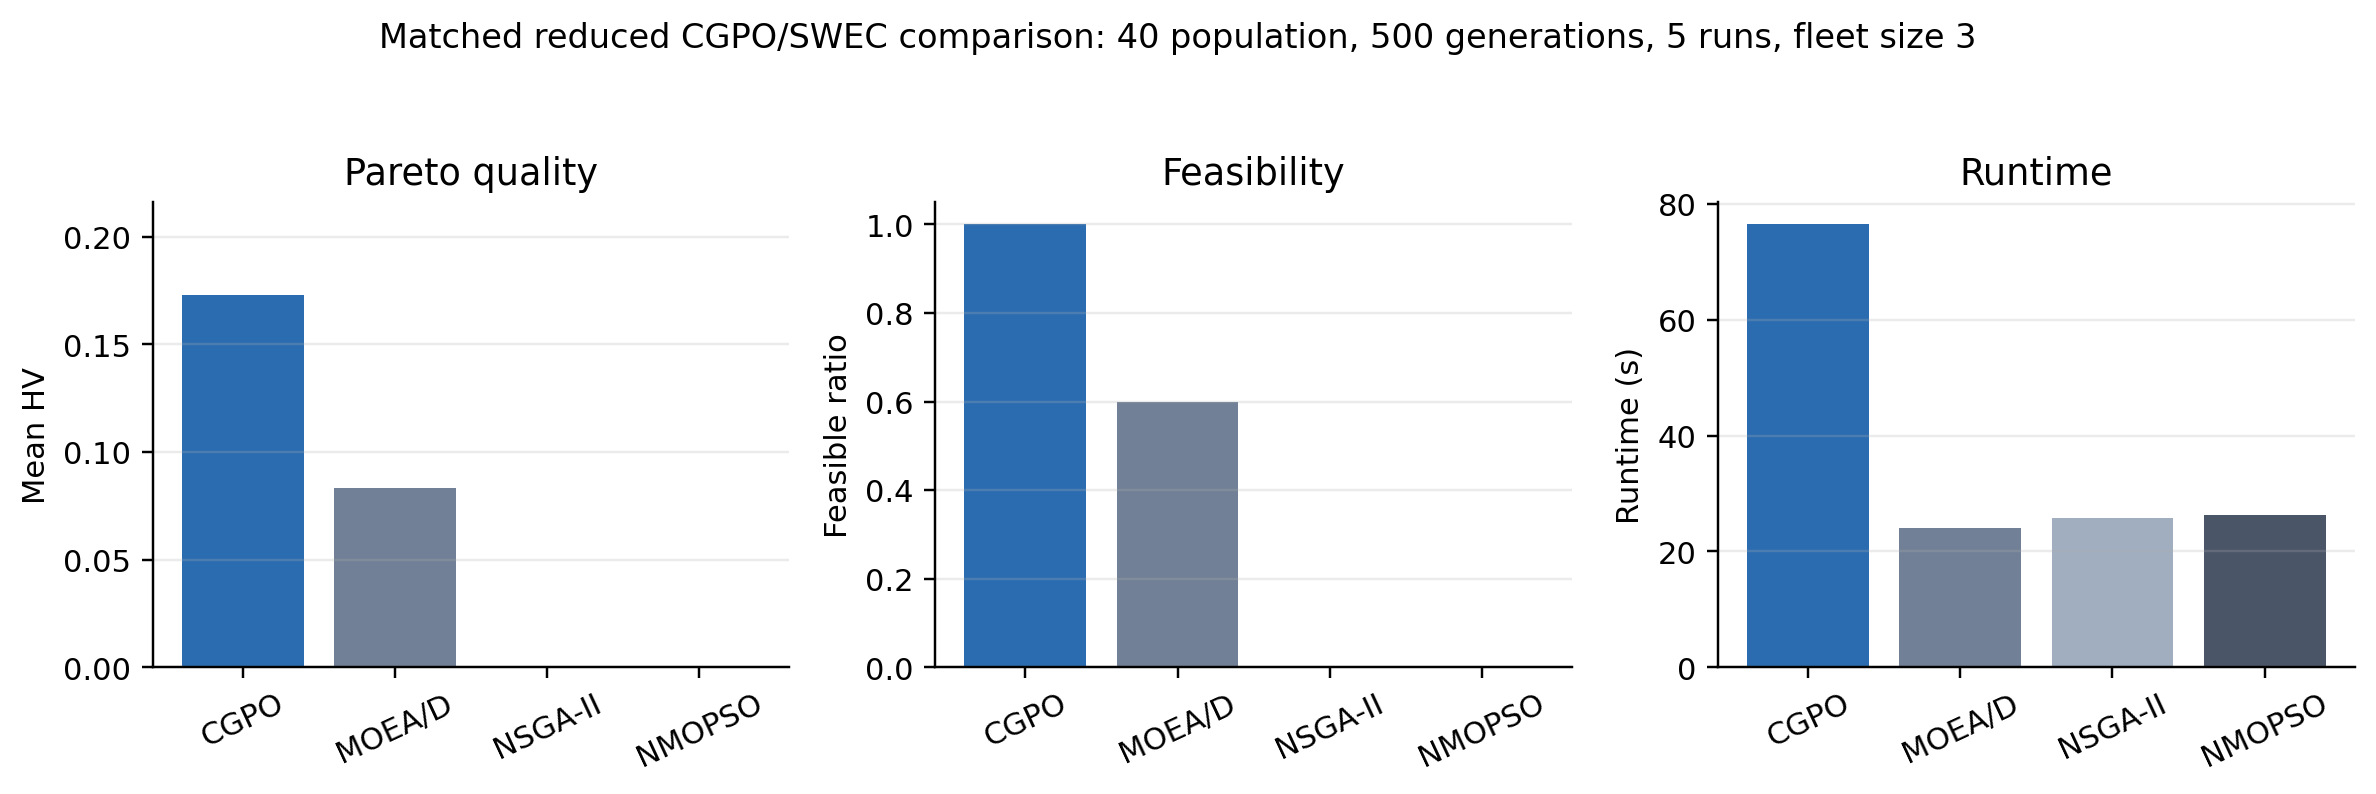
\includegraphics[width=0.96\textwidth]{figures/cgpo_matched_results_40x500_5run.png}
\caption{Data-derived reduced comparison across the three fleet-three scenarios. Bars aggregate scenario-level means from \texttt{results/cgpo\_swec\_matched\_40x500\_5run/metrics/benchmark\_metrics\_summary.csv}.}
\label{fig:matched-results}
\end{figure*}

\begin{table*}[t]
\centering
\scriptsize
\caption{Reduced matched comparison across \texttt{c\_100\_uav3}, \texttt{m\_100\_uav3}, and \texttt{s\_120\_uav3}. HV and runtime are averaged over scenario-level means; $n=5$ runs per scenario.}
\label{tab:matched-comparison}
\begin{tabular}{llrrrrrr}
\toprule
Role & Method & Runs & FR & HV & IGD+ & Conflict & Runtime \\
\midrule
Proposed & \texttt{CGPO} & 15 & 1.0000 & 0.1728 & 0.0981 & 0.0000 & 76.4872 \\
Decomposition baseline & \texttt{MOEA/D} & 15 & 0.6000 & 0.0834 & 0.2382 & 0.0000 & 24.0834 \\
Canonical MOEA baseline & \texttt{NSGA-II} & 15 & 0.0000 & 0.0000 & n/a & 0.0000 & 25.7643 \\
UAV PSO baseline & \texttt{NMOPSO} & 15 & 0.0000 & 0.0000 & n/a & 0.0001 & 26.2931 \\
\bottomrule
\end{tabular}
\end{table*}

\begin{table*}[t]
\centering
\scriptsize
\caption{Matched run-level HV comparison against CGPO. Wilcoxon tests use the alternative hypothesis that CGPO has larger HV; $p_{\mathrm{Holm}}$ applies Holm correction across the three baseline comparisons.}
\label{tab:matched-pairwise}
\begin{tabular}{lrrrrr}
\toprule
Comparison & Matched $n$ & W/T/L & Mean $\Delta$HV & Median $\Delta$HV & $p_{\mathrm{Holm}}$ \\
\midrule
CGPO vs. \texttt{MOEA/D} & 14 & 14/0/0 & 0.0841 & 0.0767 & $9.16\times10^{-5}$ \\
CGPO vs. \texttt{NSGA-II} & 15 & 15/0/0 & 0.1731 & 0.1704 & $9.16\times10^{-5}$ \\
CGPO vs. \texttt{NMOPSO} & 15 & 15/0/0 & 0.1731 & 0.1704 & $9.16\times10^{-5}$ \\
\bottomrule
\end{tabular}
\end{table*}

CGPO is the only method that returns feasible populations in every matched run. It has the best scenario-level HV rank on all three fleet-three scenarios and wins every available matched run-level HV comparison against the three reduced baselines. MOEA/D is the strongest non-CGPO baseline in this reduced protocol, but it fails the city fleet-three case and uses 35 NBI weight vectors for the requested population 40. NSGA-II and NMOPSO do not produce feasible final populations under the same budget, which makes their HV zero after feasible-mask filtering. These findings support a reduced-budget claim that CGPO is more reliable under the tested constrained fleet setting; they do not yet replace the larger planned protocol with UAV-specialized and MAPF baselines.

\subsection{Full-budget CGPO validation runs}

Two single-run full-budget inspections are available from the focused table protocol \texttt{configs/cgpo\_swec\_inspection\_40x500\_1run.yaml}. Both use 500 generations, population 40, seed 11, GPU mode off, \texttt{s\_120}, hard collision constraints, \texttt{separationMin = 10.0}, \texttt{maxTurnDeg = 75.0}, \texttt{safeDist = 20.0}, \texttt{droneSize = 1.0}, and \texttt{nRep = 40}. They are useful for implementation and feasibility inspection, but they are not statistically meaningful because each has only one run and no baseline counterpart.

\begin{table*}[t]
\centering
\scriptsize
\caption{Completed full-budget CGPO validation runs. These values support implementation and feasibility inspection; broader comparative claims require the complete multi-run protocol.}
\label{tab:inspection}
\begin{tabular}{llrrrrrrrrrr}
\toprule
Directory & Problem & Runs & FR & Success & HV & IGD+ & Runtime & Clearance & Turn & Conflict & Energy \\
\midrule
\texttt{cgpo\_swec\_inspection\_40x500\_1run} & \texttt{s\_120\_uav3} & 1 & 1.0 & 1.0 & 0.3006 & 0.0000 & 74.2049 & 3.7876 & 74.9551 & 0.0 & 0.1192 \\
\texttt{cgpo\_swec\_inspection\_40x500\_1run} & \texttt{s\_120\_uav8} & 1 & 1.0 & 1.0 & 0.0442 & 0.0000 & 214.1621 & 1.3278 & 61.3503 & 0.0 & 0.0701 \\
\bottomrule
\end{tabular}
\end{table*}

These runs show that the current CGPO implementation can complete full-budget \texttt{s\_120} fleet inspections and produce feasible reported outputs in the tested seeds. Under the 40-population table protocol, the three-UAV run achieved HV 0.3006 and the eight-UAV run achieved HV 0.0442; both reported feasible ratio 1.0, run success 1.0, and zero mission conflict rate.

The runtime difference between the two inspections is consistent with the fleet-size burden: the \texttt{s\_120\_uav8} inspection took 214.1621 seconds compared with 74.2049 seconds for \texttt{s\_120\_uav3}. This observation is an implementation diagnostic rather than a formal complexity result, because it is based on one run per fleet size.

\subsection{Ablation harness validation}

Table~\ref{tab:focused-ablation} reports a focused one-run ablation on \texttt{s\_120\_uav3}. Each variant uses 500 generations, population 40, seed 11, GPU mode off, and the same mission constraints as the validation table. The results are real benchmark outputs, but they remain descriptive because there is only one run per variant.

\begin{table*}[t]
\centering
\scriptsize
\caption{Focused 40-population, 500-generation, one-run ablation on \texttt{s\_120\_uav3}. Values are descriptive single-run results.}
\label{tab:focused-ablation}
\begin{tabular}{lrrrrrrrr}
\toprule
Variant & Runs & FR & HV mean & IGD+ mean & Runtime & Clearance & Turn & Conflict \\
\midrule
\texttt{CGPO\_full} & 1 & 1.0 & 0.4540 & 0.0514 & 73.7439 & 3.7876 & 74.9551 & 0.0 \\
\texttt{CGPO\_random\_only} & 1 & 1.0 & 0.3676 & 0.1927 & 47.3363 & 3.8462 & 66.2798 & 0.0 \\
\texttt{CGPO\_no\_cig\_edge\_coupling} & 1 & 1.0 & 0.4590 & 0.0480 & 60.6004 & 1.4211 & 71.0968 & 0.0 \\
\texttt{CGPO\_no\_ppf\_pressure} & 1 & 1.0 & 0.4639 & 0.0358 & 74.3816 & 3.7876 & 46.9165 & 0.0 \\
\texttt{CGPO\_no\_ovo\_variation} & 1 & 1.0 & 0.3182 & 0.2129 & 69.0420 & 3.5678 & 74.5429 & 0.0 \\
\texttt{CGPO\_no\_ovo\_fleet\_coordination} & 1 & 1.0 & 0.4479 & 0.0446 & 71.5178 & 3.8462 & 59.0840 & 0.0 \\
\bottomrule
\end{tabular}
\end{table*}

\section{Ablation and trace analysis}
\label{sec:ablation}

\subsection{Trace signals exposed by the lean three-mechanism CGPO}

The trace harness records, per generation and per variant, mean and per-UAV CIG tension, terrain-edge count, turn-edge count, pairwise-edge count, smoothing-edge count, conflict-cluster count, PPF feasibility pressure, exploration scale, boundary mass, feasible mass, pressure entropy, OVO perturbation scale, perturbed waypoint count, coordinated cluster count, and parent-blend entropy. The expected, code-pinned response of these signals to the ablation switches is: when CIG edge coupling is disabled, pairwise and smoothing edge counts drop to zero and PPF tension input flattens; when PPF pressure is disabled, parent selection becomes uniform and the feasibility-pressure and pressure-entropy series degenerate; when OVO variation is disabled, the perturbation scale and parent-blend entropy series drop to zero; and when only the OVO fleet-coordination pass is disabled, the coordinated-cluster count drops to zero while the rest of the OVO trace remains active. The full ablation analysis script verifies this code-pinned mapping and reports it alongside the external metrics so that any external degradation can be linked back to the correct internal mechanism.

\subsection{Ablation interpretation rule}

Ablations should be interpreted by external metrics first and traces second. In the reduced one-run ablation, disabling OVO variation clearly reduces HV and worsens IGD+, while disabling CIG edge coupling or PPF pressure does not degrade this single \texttt{s\_120\_uav3} case. These results make OVO variation the best-supported component in the reduced evidence and make CIG/PPF conditional mechanisms that need broader multi-scenario ablation before stronger necessity claims. If a trace changes but the external metrics do not improve, the mechanism should be presented as inspectable but not necessary. If a removed component improves external metrics, the method should be simplified rather than defended by terminology.

\section{Reproducibility}
\label{sec:reproducibility}

The repository contains the configs and result-artifact conventions needed for reproduction. The reduced matched comparison, focused fleet-size inspection, and focused ablation are controlled by the three CGPO/SWEC 40x500 YAML configs under \texttt{configs/}. The matched-comparison command writes benchmark manifests, raw per-run artifacts, metric summaries, pairwise statistics, rank summaries, table CSVs, and the data-derived result figure.

The result bundle should include benchmark manifests, config files, raw per-run artifacts, metric summaries, pairwise statistics, win/tie/loss summaries, ablation summaries, trace summaries, figure source data, and the final manuscript.

The completed 40-population inspection manifest records macOS arm64, Python 3.10.19, NumPy 2.2.6, SciPy 1.15.3, repository branch \texttt{codex/repo-hygiene-and-fixes}, commit \texttt{8d30d19d}, and a dirty working tree. A clean submission should record the final commit hash and whether the result directory was generated from a clean or dirty tree.

\section{Limitations}
\label{sec:limitations}

The study has four important limitations. First, the completed numerical evidence is a reduced comparative benchmark, not the full planned protocol. It includes a five-run matched comparison against NSGA-II, MOEA/D, and NMOPSO on three fleet-three scenarios, plus focused single-run fleet-size and ablation inspections. This supports reduced-budget claims against these baselines, but it does not support broad state-of-the-art claims across UAV-specialized or MAPF-style methods. MOEA/D also generated 35 NBI weight vectors for the requested population of 40, so that detail should be retained when interpreting its row.

Second, the benchmark is simulation-centered and static. It does not model online replanning, wind, communication loss, onboard controller dynamics, hardware-in-the-loop validation, or real-flight execution.

Third, equal generations and population do not guarantee perfectly equal objective-evaluation counts for all algorithms. The lean three-mechanism CGPO uses one full mission evaluation per offspring and no projection-proxy evaluations. The paper records candidate evaluations and total mission-evaluation calls in run metadata and reports these counts next to runtime whenever CGPO is compared with baselines.

Fourth, CGPO has computational overhead. The 40-population full-budget single-run inspection on \texttt{s\_120\_uav8} took 214.1621 seconds on the recorded local environment. Runtime must therefore remain part of the final quality discussion.

\section{Conclusion}
\label{sec:conclusion}

This paper presents CGPO, a constraint-graph policy optimizer for constrained multi-UAV multi-objective path planning. The published method uses a dynamic constraint-interaction graph to connect Pareto pressure-field selection and orchestrated fleet-aware variation, with no explicit feasibility projection, repair stack, constructive route priors, or matched hybrid baselines in the active repository implementation. The repository exposes the relevant control paths and trace variables, and the SWEC-style protocol specifies the terrain cases, baselines, budgets, metrics, statistics, and ablations needed for a defensible evaluation.

The completed reduced-budget artifacts show that CGPO returns feasible populations in all matched fleet-three runs and outperforms NSGA-II, MOEA/D, and NMOPSO on matched HV comparisons under the tested budget. The focused fleet-size inspection confirms that CGPO can complete \texttt{s\_120} three- and eight-UAV runs with zero reported mission conflict rate. The one-run ablation supports OVO variation as the clearest contributor in the tested case, while CIG and PPF remain conditional mechanisms requiring broader ablation evidence.

\section*{Data and code availability}

The manuscript is based on the local UAV benchmark repository. The active reduced-budget paper configs are the matched comparison, inspection, and ablation CGPO/SWEC YAML files under \texttt{configs/}. The CGPO implementation is under \texttt{uav\_benchmark/algorithms/cgpo/}. The completed numerical artifacts are stored in the corresponding CGPO/SWEC result directories and summarized in the paper-artifact manifest.

\section*{Declaration of generative AI and AI-assisted technologies}

During manuscript preparation, AI-assisted writing tools were used to help organize and edit text. All scientific claims, numerical values, and artifact references were checked against local repository files and result outputs by the authors.

\bibliographystyle{../../template/els-cas-templates/cas-model2-names}
\bibliography{cgpo_swec_refs}

\end{document}
